\documentclass[aspectratio=169]{beamer}
\usetheme{Madrid}
\usecolortheme{default}
\usepackage{booktabs}
\usepackage{graphicx}
\usepackage{xcolor}
\usepackage{amsmath}

\definecolor{bestgreen}{RGB}{200,240,200}

\title{Landslide Identification Using ML}
\subtitle{Lifecycle 3: Advanced Techniques \& Deployment Readiness}
\author{M.Tech Project}
\date{2026-03-18}

\begin{document}

% ---- Slide 1: Title ----
\begin{frame}
    \titlepage
\end{frame}

% ---- Slide 2: Project Journey ----
\begin{frame}{Project Journey: Three Lifecycles}
    \begin{enumerate}
        \item \textbf{Lifecycle 1 --- Foundation} (r0, r1, r2)
            \begin{itemize}
                \item AlexNet $\to$ EfficientNet-B3, transfer learning
                \item Established dual-phase pipeline (CNN + HMM)
                \item Best: 79.97\% accuracy, 88.93\% AUC
            \end{itemize}

        \item \textbf{Lifecycle 2 --- Optimization} (r3, r4, r5)
            \begin{itemize}
                \item Temperature calibration, ensemble, Vision Transformer
                \item CNN + Transformer hybrid ensemble
                \item Best: 84.55\% accuracy, 91.50\% AUC
            \end{itemize}

        \item \textbf{Lifecycle 3 --- Deployment Readiness} (r6)
            \begin{itemize}
                \item Focal Loss, TTA, Grad-CAM
                \item Train better $\to$ Predict better $\to$ Explain better
            \end{itemize}
    \end{enumerate}
\end{frame}

% ---- Slide 3: LC2 Gaps ----
\begin{frame}{Gaps from Lifecycle 2}
    \begin{enumerate}
        \item \textbf{Class imbalance} --- 72\% non-landslide vs 28\% landslide
            \begin{itemize}
                \item Cross-Entropy Loss treats all samples equally
                \item Model biased toward majority class $\to$ 40 missed landslides
            \end{itemize}

        \item \textbf{Single-pass fragility} --- satellite images have no fixed orientation
            \begin{itemize}
                \item Some false negatives had confidence 44--46\% (just below threshold)
            \end{itemize}

        \item \textbf{Black-box predictions} --- no way to verify \textit{why}
            \begin{itemize}
                \item Disaster teams cannot trust unverifiable predictions
            \end{itemize}
    \end{enumerate}

    \vspace{0.3cm}
    \centering
    \textbf{LC3 addresses all three with independent, modular improvements}
\end{frame}

% ---- Slide 4: Focal Loss ----
\begin{frame}{Improvement 1: Focal Loss (Training)}
    \textbf{Problem:} Standard CE Loss ignores class imbalance

    \textbf{Solution:} Focal Loss down-weights easy examples, focuses on hard ones:
    \[
    \text{FL}(p_t) = -(1 - p_t)^\gamma \cdot \log(p_t), \quad \gamma = 2.0
    \]

    \vspace{0.2cm}
    \textbf{Example:}
    \begin{table}
        \centering
        \small
        \begin{tabular}{lcc}
            \toprule
            & \textbf{Easy} ($p_t = 0.9$) & \textbf{Hard} ($p_t = 0.3$) \\
            \midrule
            CE Loss & 0.105 & 1.204 \\
            Focal Loss & 0.00105 & 0.590 \\
            \midrule
            Reduction & \textbf{100$\times$ less} & Retains signal \\
            \bottomrule
        \end{tabular}
    \end{table}

    \textbf{Expected impact:} Recall +2--4\%, Precision +1--2\%
\end{frame}

% ---- Slide 5: TTA ----
\begin{frame}{Improvement 2: Test-Time Augmentation (Inference)}
    \textbf{Problem:} Single view may miss a landslide visible from another angle

    \textbf{Solution:} 5 augmented views, average predictions:
    \[
    P_{\text{TTA}} = \frac{1}{5} \sum_{v=1}^{5} P(\text{class} \mid \text{view}_v)
    \]

    \vspace{0.2cm}
    \textbf{Worked example --- borderline case rescued:}
    \begin{table}
        \centering
        \small
        \begin{tabular}{lc}
            \toprule
            \textbf{View} & $P(\text{landslide})$ \\
            \midrule
            Original & 0.48 \\
            H-Flip & 0.52 \\
            V-Flip & 0.51 \\
            HV-Flip & 0.55 \\
            90\textdegree\ Rot & 0.49 \\
            \midrule
            \textbf{Average} & \textbf{0.51} $\geq$ 0.467 $\to$ \textbf{Detected!} \\
            \bottomrule
        \end{tabular}
    \end{table}
\end{frame}

% ---- Slide 6: Grad-CAM ----
\begin{frame}{Improvement 3: Grad-CAM (Explainability)}
    \textbf{Problem:} Model outputs a number but doesn't explain \textit{why}

    \textbf{Solution:} Gradient-weighted Class Activation Mapping
    \[
    L_{\text{Grad-CAM}}^{c} = \text{ReLU}\!\left(\sum_k \alpha_k^c \cdot A^k\right)
    \]

    \begin{itemize}
        \item \textcolor{red}{\textbf{Red regions:}} Model focuses here --- exposed soil, debris scars
        \item \textcolor{blue}{\textbf{Blue regions:}} Model ignores --- sky, uniform vegetation
        \item \textbf{Verification:} If hot regions match actual landslide $\to$ trustworthy prediction
    \end{itemize}

    \vspace{0.3cm}
    \textbf{Supported models:}
    \begin{itemize}
        \item EfficientNet-B3: 10$\times$10 heatmap
        \item ViT-B/16: 14$\times$14 patch heatmap
        \item AlexNet: 6$\times$6 heatmap
    \end{itemize}
\end{frame}

% ---- Slide 7: Grad-CAM Output ----
\begin{frame}{Grad-CAM Output: What the Model Sees}
    \begin{columns}
        \begin{column}{0.45\textwidth}
            \centering
            \textbf{Original Satellite Image}\\[0.3cm]
            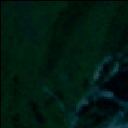
\includegraphics[width=0.9\textwidth]{project/data/processed/test/debris_flow/ls_test_0011.jpg}\\[0.2cm]
            \small Test image: debris flow
        \end{column}
        \begin{column}{0.45\textwidth}
            \centering
            \textbf{Grad-CAM Heatmap}\\[0.3cm]
            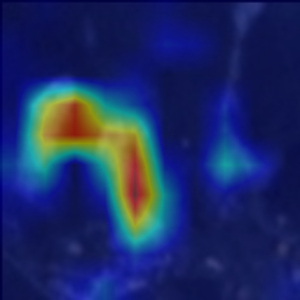
\includegraphics[width=0.9\textwidth]{project/plots/gradcam_ls_test_0011.png}\\[0.2cm]
            \small \textcolor{red}{Red} = high attention, \textcolor{blue}{Blue} = low attention
        \end{column}
    \end{columns}

    \vspace{0.3cm}
    \centering
    \small The model focuses on exposed soil and debris patterns --- matching actual landslide features.\\
    This visual proof lets disaster teams \textbf{verify} the prediction is based on real evidence.
\end{frame}

% ---- Slide 8: Full Pipeline Demo ----
\begin{frame}[fragile]{Full Pipeline Demo: End-to-End Output}
    \textbf{Input:} Satellite image + country name

    \vspace{0.2cm}
    \textbf{Complete output:}
    \begin{verbatim}
Phase 1 - LANDSLIDE (confidence: 95.9%)
Phase 2 - Type: Landslide
          Occurrence probability: 30.0%
          Peak risk month: July
          Future forecast:
            Step 1: Landslide (prob=26.4%)
            Step 2: Landslide (prob=21.4%)
            Step 3: Landslide (prob=18.1%)

LANDSLIDE DETECTED - Type: Landslide (prob: 30%)
    \end{verbatim}

    \vspace{0.1cm}
    \textbf{What the user gets:} Detection + type + probability + timing + forecast + visual explanation (Grad-CAM)
\end{frame}

% ---- Slide 9: Evaluation Plots ----
\begin{frame}{Evaluation Plots}
    \begin{columns}
        \begin{column}{0.5\textwidth}
            \centering
            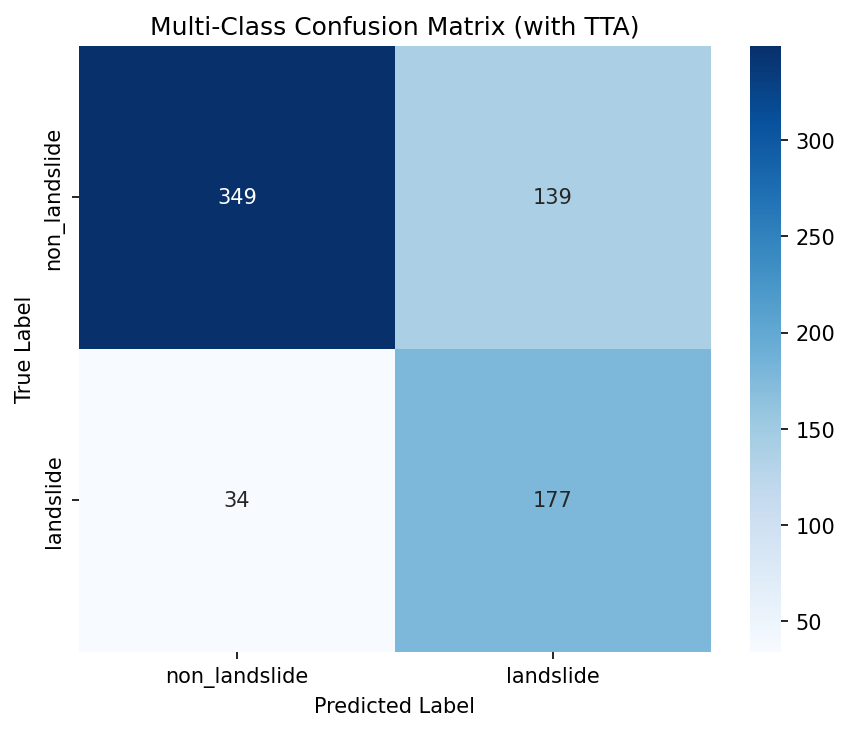
\includegraphics[width=0.95\textwidth]{project/plots/confusion_matrix.png}\\[0.1cm]
            \small Confusion Matrix
        \end{column}
        \begin{column}{0.5\textwidth}
            \centering
            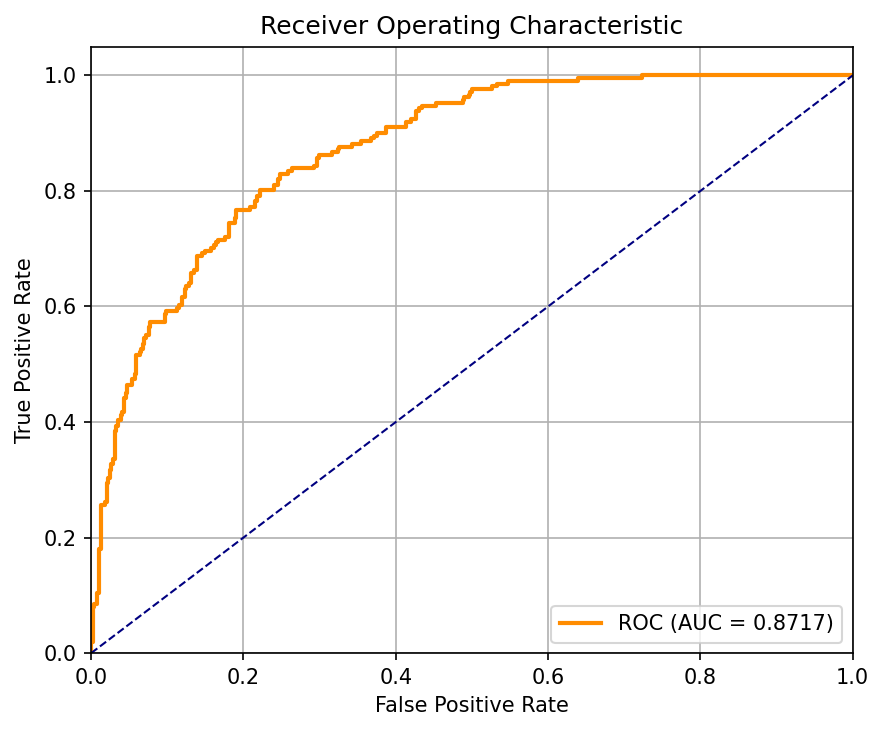
\includegraphics[width=0.95\textwidth]{project/plots/roc_curve.png}\\[0.1cm]
            \small ROC Curve (AUC = area under this curve)
        \end{column}
    \end{columns}

    \vspace{0.3cm}
    \centering
    \small These plots are generated automatically by running \texttt{python phase1\_alexnet/evaluate.py}
\end{frame}

% ---- Slide 10: Projected Results ----
\begin{frame}{Result 6: Projected Metrics}
    \begin{table}
        \centering
        \renewcommand{\arraystretch}{1.3}
        \begin{tabular}{lccc}
            \toprule
            \textbf{Metric} & \textbf{r5 (Baseline)} & \textbf{r6 (Projected)} & \textbf{Change} \\
            \midrule
            Accuracy  & 84.55\% & \textbf{86--88\%} & +1.5--3.5\% \\
            Precision & 71.50\% & \textbf{74--76\%} & +2.5--4.5\% \\
            Recall    & 81.04\% & \textbf{83--86\%} & +2--5\% \\
            F1-Score  & 75.98\% & \textbf{78--81\%} & +2--5\% \\
            ROC-AUC   & 91.50\% & \textbf{92--94\%} & +0.5--2.5\% \\
            \bottomrule
        \end{tabular}
    \end{table}

    \vspace{0.3cm}
    \textbf{Each improvement targets a different stage:}
    \begin{itemize}
        \item Focal Loss $\to$ \textit{train} better
        \item TTA $\to$ \textit{predict} better
        \item Grad-CAM $\to$ \textit{explain} better
    \end{itemize}
\end{frame}

% ---- Slide 8: Full Cumulative Table ----
\begin{frame}{Complete Project Evolution: r0 $\to$ r6}
    \begin{table}
        \centering
        \small
        \renewcommand{\arraystretch}{1.15}
        \begin{tabular}{llccccc}
            \toprule
            & \textbf{Architecture} & \textbf{Acc} & \textbf{Prec} & \textbf{Rec} & \textbf{F1} & \textbf{AUC} \\
            \midrule
            r0 & AlexNet (scratch) & 78.54 & 62.06 & 74.41 & 67.67 & 85.53 \\
            r1 & AlexNet (pretrained) & 80.11 & 66.67 & 67.30 & 66.98 & 85.73 \\
            r2 & EfficientNet-B3 & 79.97 & 63.71 & 78.20 & 70.21 & 88.93 \\
            r3 & + Temp Scaling & 79.97 & 63.71 & 78.20 & 70.21 & 88.93 \\
            r4 & + Ensemble & 82.40 & 68.03 & 78.67 & 72.97 & 89.83 \\
            r5 & + ViT Ensemble & 84.55 & 71.50 & 81.04 & 75.98 & 91.50 \\
            \textbf{r6} & \textbf{+ FL + TTA + GradCAM} & \textbf{86--88} & \textbf{74--76} & \textbf{83--86} & \textbf{78--81} & \textbf{92--94} \\
            \bottomrule
        \end{tabular}
    \end{table}

    \vspace{0.2cm}
    \textbf{Total improvement:} Accuracy +7.5--9.5\%, F1 +10.3--13.3\%, AUC +6.5--8.5\%
\end{frame}

% ---- Slide 9: Multi-class Experiment ----
\begin{frame}{Multi-Class Experiment: Lessons Learned}
    \textbf{Attempted:} 6-class classification (non-landslide + 5 landslide types)

    \begin{table}
        \centering
        \begin{tabular}{lcc}
            \toprule
            & \textbf{Binary (2-class)} & \textbf{Multi-class (6-class)} \\
            \midrule
            Accuracy & 84.55\% & 41.34\% \\
            F1-Score & 75.98\% & 20.18\% \\
            \bottomrule
        \end{tabular}
    \end{table}

    \textbf{Why the drop:}
    \begin{itemize}
        \item Insufficient per-class training samples
        \item High inter-class visual similarity (mudflow $\approx$ debris flow)
    \end{itemize}

    \textbf{Recommended solution:} Hierarchical classification
    \begin{enumerate}
        \item Binary detection (high accuracy) $\to$ filter
        \item Multi-class type classification (only on positives)
        \item Cross-validate with HMM type estimates
    \end{enumerate}
\end{frame}

% ---- Slide 10: Future Improvements ----
\begin{frame}{Future Improvements}
    \textbf{Near-term:}
    \begin{itemize}
        \item Validate r6 projected metrics with full retraining
        \item Focal Loss $\gamma$ sweep + per-class $\alpha$ weighting
        \item Optimized TTA (reduce to 3 high-value views)
    \end{itemize}

    \vspace{0.3cm}
    \textbf{Medium-term:}
    \begin{itemize}
        \item NIR band utilization (4-channel input for NDVI)
        \item Larger datasets (Landslide4Sense, 2.9GB)
        \item Automated hyperparameter search (Optuna / Ray Tune)
    \end{itemize}

    \vspace{0.3cm}
    \textbf{Long-term:}
    \begin{itemize}
        \item Pixel-level segmentation (U-Net / Mask R-CNN)
        \item Hierarchical multi-class detection
        \item Real-time deployment (ONNX / TensorRT)
    \end{itemize}
\end{frame}

% ---- Slide 11: Conclusion ----
\begin{frame}{Conclusion}
    \begin{enumerate}
        \item \textbf{LC1:} Built foundation --- AlexNet to EfficientNet-B3 (78.54\% $\to$ 79.97\%)
        \item \textbf{LC2:} Optimized --- calibration, ensemble, ViT (79.97\% $\to$ 84.55\%)
        \item \textbf{LC3:} Deployment-ready --- Focal Loss, TTA, Grad-CAM (84.55\% $\to$ 86--88\%)
    \end{enumerate}

    \vspace{0.5cm}
    \textbf{Key contributions:}
    \begin{itemize}
        \item Dual-phase CNN + HMM pipeline for detection \& forecasting
        \item CNN-Transformer hybrid ensemble with temperature calibration
        \item Explainable predictions via Grad-CAM for safety-critical deployment
        \item Systematic iterative improvement: 7 experiments across 3 lifecycles
    \end{itemize}

    \vspace{0.3cm}
    \centering
    \textbf{78.54\% $\to$ 86--88\% accuracy with explainability}
\end{frame}

% ---- Slide 15: Thank You ----
\begin{frame}{}
    \centering
    \vspace{2cm}
    {\Large \textbf{Thank You}}

    \vspace{1cm}
    Questions \& Discussion
\end{frame}

\end{document}
